\documentclass[11pt]{article}
\usepackage[margin=1in]{geometry}
\usepackage[T1]{fontenc}
\usepackage[utf8]{inputenc}
\usepackage{lmodern}
\usepackage{amsmath,amssymb}
\usepackage{amsthm}
\usepackage{tikz}
\usetikzlibrary{arrows.meta}
\tikzset{root/.style={draw,circle,thick}}

\newtheorem{definition}{Definition}
\newtheorem{example}{Example}
\newtheorem{remark}{Remark}
\newtheorem{theorem}{Theorem}

\title{Incremental Fixpoint Computation:\\A Two-Level Architecture}
\author{}
\date{}

\begin{document}
\maketitle

\tableofcontents
\bigskip

\begin{abstract}
We observe that the incremental dead code elimination (DCE) algorithm from our reactive DCE work is an instance of a more general pattern: \emph{incremental fixpoint computation}.
This note proposes a two-level architecture for incremental fixpoints:
(1)~a low-level API that assumes user-provided incremental operations, and
(2)~a potential high-level DSL where these operations are derived automatically from a structured definition of the fixpoint operator.
The relationship between these levels is analogous to that between manual gradient computation and automatic differentiation.
\end{abstract}

\section{Motivation: DCE as Incremental Fixpoint}

In reactive DCE, the live set is defined as the least fixpoint of a monotone operator:
\[
F_G(S) = G.\mathsf{roots} \cup \{ v \mid \exists u \in S.\, (u,v) \in G.\mathsf{edges} \}
\]
That is, $\mathsf{liveSet}(G) = \mathsf{lfp}(F_G)$.

When the graph changes ($G \to G' = G \pm f$), we want to update the fixpoint incrementally rather than recomputing from scratch.
The key observations are:
\begin{itemize}
  \item \textbf{Expansion} ($G \to G \oplus f$): The operator grows, so $\mathsf{lfp}(F_G) \subseteq \mathsf{lfp}(F_{G'})$. The old fixpoint is an underapproximation; we iterate upward.
  \item \textbf{Contraction} ($G \to G \ominus f$): The operator shrinks, so $\mathsf{lfp}(F_{G'}) \subseteq \mathsf{lfp}(F_G)$. The old fixpoint is an overapproximation; we must remove unjustified elements.
\end{itemize}

This pattern---incremental maintenance of a least fixpoint under changes to the underlying operator---arises in many domains beyond DCE.

\section{The General Pattern}

\begin{definition}[Monotone Fixpoint Problem]
Given a complete lattice $(L, \sqsubseteq)$ and a monotone operator $F : L \to L$, the \emph{least fixpoint} is $\mathsf{lfp}(F) = \bigcap \{ x \mid F(x) \sqsubseteq x \}$.
\end{definition}

For set-based fixpoints (our focus), $L = \mathcal{P}(A)$ for some element type $A$, ordered by $\subseteq$, and $F$ is typically of the form:
\[
F(S) = \mathsf{base} \cup \mathsf{step}(S)
\]
where $\mathsf{base}$ provides seed elements and $\mathsf{step}$ derives new elements from existing ones.

\begin{definition}[Incremental Fixpoint Problem]
Given:
\begin{itemize}
  \item A current fixpoint $S = \mathsf{lfp}(F)$
  \item A change that transforms $F$ into $F'$
\end{itemize}
Compute $S' = \mathsf{lfp}(F')$ efficiently, in time proportional to $|S' \triangle S|$ rather than $|S'|$.
\end{definition}

\section{Level 1: Low-Level Incremental Fixpoint API}

%%%%%%%%%%%%%%%%%%%%%%%%%%%%%%%%%%%%%%%%%%%%%%%%%%%%%%%%%%%%%%%%%%%%%%%%%%%%%%%
\subsection{API Specification}
%%%%%%%%%%%%%%%%%%%%%%%%%%%%%%%%%%%%%%%%%%%%%%%%%%%%%%%%%%%%%%%%%%%%%%%%%%%%%%%

\begin{remark}[Two API Levels]
The API has two levels depending on which operations are needed:
\begin{itemize}
\item \textbf{Simple API} (expansion only): Supports adding elements to base or edges.
      Requires only $\mathsf{base}$ and $\mathsf{stepFwd}$.
\item \textbf{Full API} (expansion + contraction): Also supports removing elements.
      Additionally requires $\mathsf{stepInv}$ and $\mathsf{rank}$.
\end{itemize}
Many applications only need expansion (e.g., monotonically growing graphs). The simple API suffices and is easier to implement.
\end{remark}

\subsubsection{Types}

\begin{center}
\begin{tabular}{ll}
$A$ & Element type (e.g., graph nodes) \\
$\mathsf{Set}(A)$ & Finite sets of elements \\
$\mathsf{Map}(A, \mathbb{N})$ & Map from elements to natural numbers (ranks)
\end{tabular}
\end{center}

\subsubsection{Configuration (User Provides)}

\begin{center}
\begin{tabular}{lp{6.5cm}l}
$\mathsf{base} : \mathsf{Set}(A)$ & Seed elements (e.g., roots) & required \\
$\mathsf{stepFwd} : A \to \mathsf{Set}(A)$ & Forward derivation & required \\
$\mathsf{stepInv} : A \to \mathsf{Set}(A)$ & Inverse derivation & for contraction
\end{tabular}
\end{center}

\medskip
\noindent Define $\mathsf{step}(S) = \bigcup_{x \in S} \mathsf{stepFwd}(x)$ and $F(S) = \mathsf{base} \cup \mathsf{step}(S)$.

\medskip
\noindent \textbf{Note:} If $\mathsf{stepInv}$ is not provided, the system can build it from $\mathsf{stepFwd}$:
\[
\mathsf{stepInv}[y] = \{ x \in \mathsf{current} \mid y \in \mathsf{stepFwd}(x) \}
\]
This is computed once during initialization and maintained incrementally.

\subsubsection{State (System Maintains)}

\begin{center}
\begin{tabular}{lp{6.5cm}l}
$\mathsf{current} : \mathsf{Set}(A)$ & Current live set $= \mathsf{lfp}(F)$ & always \\
$\mathsf{rank} : \mathsf{Map}(A, \mathbb{N})$ & BFS distance from base & for contraction
\end{tabular}
\end{center}

\subsubsection{Required Properties}

\begin{enumerate}
\item \textbf{stepInv correctness} (if provided): $y \in \mathsf{stepInv}(x) \Leftrightarrow x \in \mathsf{stepFwd}(y)$
\item \textbf{Element-wise} (automatic): $\mathsf{step}$ decomposes via $\mathsf{stepFwd}$
\item \textbf{Additive} (automatic): $\mathsf{step}(A \cup B) = \mathsf{step}(A) \cup \mathsf{step}(B)$
\end{enumerate}

\begin{example}[DCE Instance]
\begin{align*}
\mathsf{base} &= \mathsf{roots} \\
\mathsf{stepFwd}(u) &= \{ v \mid (u, v) \in \mathsf{edges} \} \quad \text{(successors)} \\
\mathsf{stepInv}(v) &= \{ u \mid (u, v) \in \mathsf{edges} \} \quad \text{(predecessors, optional)}
\end{align*}
\end{example}

%%%%%%%%%%%%%%%%%%%%%%%%%%%%%%%%%%%%%%%%%%%%%%%%%%%%%%%%%%%%%%%%%%%%%%%%%%%%%%%
\subsection{Algorithms}
%%%%%%%%%%%%%%%%%%%%%%%%%%%%%%%%%%%%%%%%%%%%%%%%%%%%%%%%%%%%%%%%%%%%%%%%%%%%%%%

\subsubsection{Expansion (BFS)}

When the operator grows ($F \sqsubseteq F'$: base or edges added), propagate new elements:

\begin{verbatim}
expand(state, config'):
  frontier = config'.base \ state.current
  r = 0
  while frontier != {}:
    for x in frontier:
      state.current.add(x)
      state.rank[x] = r
    nextFrontier = {}
    for x in frontier:
      for y in config'.stepFwd(x):
        if y not in state.current:
          nextFrontier.add(y)
    frontier = nextFrontier
    r += 1
\end{verbatim}

\subsubsection{Contraction (Worklist Cascade)}

When the operator shrinks ($F' \sqsubseteq F$: base or edges removed), remove unsupported elements:

\begin{verbatim}
contract(state, config'):
  // Initialize: nodes that lost base membership or an incoming edge
  worklist = { x | x lost support }
  dying = {}

  while worklist != {}:
    x = worklist.pop()
    if x in dying or x in config'.base: continue

    // Check for well-founded deriver (strictly lower rank)
    hasSupport = false
    for y in config'.stepInv(x):
      if y in (state.current \ dying) and state.rank[y] < state.rank[x]:
        hasSupport = true
        break

    if not hasSupport:
      dying.add(x)
      // Notify dependents
      for z where x in config'.stepInv(z):
        worklist.add(z)

  state.current -= dying
\end{verbatim}

\subsubsection{Why Ranks Break Cycles}

The rank check $\mathsf{rank}[y] < \mathsf{rank}[x]$ is essential:
\begin{itemize}
\item Cycle members have \emph{equal} ranks (same BFS distance from base)
\item Therefore, they cannot provide well-founded support to each other
\item An unreachable cycle has no well-founded support and is correctly removed
\end{itemize}

%%%%%%%%%%%%%%%%%%%%%%%%%%%%%%%%%%%%%%%%%%%%%%%%%%%%%%%%%%%%%%%%%%%%%%%%%%%%%%%
\subsection{Correctness and Analysis}
%%%%%%%%%%%%%%%%%%%%%%%%%%%%%%%%%%%%%%%%%%%%%%%%%%%%%%%%%%%%%%%%%%%%%%%%%%%%%%%

\subsubsection{Proven Properties (Lean, all complete)}

\begin{theorem}[Expansion Correctness]
If $F \sqsubseteq F'$ and expansion terminates, then $\mathsf{current} = \mathsf{lfp}(F')$.
\end{theorem}

\begin{theorem}[Contraction Correctness]
If $F' \sqsubseteq F$ and contraction terminates, then $\mathsf{current} = \mathsf{lfp}(F')$.
\end{theorem}

\begin{theorem}[Soundness]
At all intermediate states: expansion gives $\mathsf{current} \subseteq \mathsf{lfp}(F')$; contraction gives $\mathsf{lfp}(F') \subseteq \mathsf{current}$.
\end{theorem}

All proofs complete in Lean with no \texttt{sorry}.%
\footnote{See \texttt{lean-formalisation/IncrementalFixpoint.lean}.}

\subsubsection{Complexity Analysis}

\begin{center}
\begin{tabular}{|l|c|c|}
\hline
\textbf{Operation} & \textbf{Time} & \textbf{Space} \\
\hline
Expansion & $O(|\text{new}| + |\text{edges from new}|)$ & $O(|\text{new}|)$ \\
Contraction & $O(|\text{dying}| + |\text{edges to dying}|)$ & $O(|\text{dying}|)$ \\
Rank storage & --- & $O(|\mathsf{current}|)$ integers \\
\hline
\end{tabular}
\end{center}

For DCE, this matches the complexity of dedicated graph reachability algorithms.

\subsubsection{Gap Between Proofs and Algorithms}

\begin{center}
\begin{tabular}{|l|p{5cm}|l|}
\hline
\textbf{Gap} & \textbf{Description} & \textbf{Status} \\
\hline
Refinement & Pseudo-code implements the spec & Visually obvious \\
Termination & Algorithms halt on finite sets & Clear (monotonic) \\
stepInv & User provides correct inverse & Assumed \\
\hline
\end{tabular}
\end{center}

These gaps are mechanical to close. A good engineer can implement with confidence.

%%%%%%%%%%%%%%%%%%%%%%%%%%%%%%%%%%%%%%%%%%%%%%%%%%%%%%%%%%%%%%%%%%%%%%%%%%%%%%%
\subsection{Formal Definitions (Reference)}
%%%%%%%%%%%%%%%%%%%%%%%%%%%%%%%%%%%%%%%%%%%%%%%%%%%%%%%%%%%%%%%%%%%%%%%%%%%%%%%

For completeness, the formal definitions used in Lean proofs.

\begin{definition}[Decomposed Operator]
$F(S) = B \cup \mathsf{step}(S)$ where $\mathsf{step}$ is monotone.
\end{definition}

\begin{definition}[Rank]
$\mathsf{rank}(x) = \min \{ n \mid x \in F^n(\emptyset) \}$.
\end{definition}

\begin{definition}[Well-Founded Derivation]
$y$ wf-derives $x$ if $\mathsf{rank}(y) < \mathsf{rank}(x)$ and $x \in \mathsf{step}(\{y\})$.
\end{definition}

\begin{definition}[Semi-Naive Iteration]
$C_0 = I$, $\Delta_0 = I$, $\Delta_{n+1} = \mathsf{step}(\Delta_n) \setminus C_n$, $C_{n+1} = C_n \cup \Delta_{n+1}$.
\end{definition}

\begin{definition}[Well-Founded Cascade]
$K_0 = I$, $K_{n+1} = K_n \setminus \{ x \mid x \notin B \land \text{no wf-deriver in } K_n \}$.
\end{definition}

%%%%%%%%%%%%%%%%%%%%%%%%%%%%%%%%%%%%%%%%%%%%%%%%%%%%%%%%%%%%%%%%%%%%%%%%%%%%%%%
\section{Worked Example: DCE in Detail}
%%%%%%%%%%%%%%%%%%%%%%%%%%%%%%%%%%%%%%%%%%%%%%%%%%%%%%%%%%%%%%%%%%%%%%%%%%%%%%%

We illustrate the API and algorithms with Dead Code Elimination (DCE), showing how expansion and contraction work on concrete graphs.

\subsection{Setup}

Consider a program represented as a directed graph where nodes are code units and edges represent dependencies (``$u \to v$'' means $u$ uses $v$).

\begin{center}
\begin{tikzpicture}[>=Stealth, node distance=1.6cm]
  \node[root] (R) at (0,0) {$R$};
  \node (A) at (1.8,0) {$A$};
  \node (B) at (3.6,0) {$B$};
  \node (C) at (5.4,0) {$C$};
  \node (D) at (1.8,-1.6) {$D$};

  \draw[->] (R) -- (A);
  \draw[->] (A) -- (B);
  \draw[->] (B) -- (C);
  \draw[->] (A) -- (D);
  \draw[->] (D) -- (B);
\end{tikzpicture}
\end{center}

\begin{itemize}
\item $\mathsf{base} = \{R\}$ (R is the root/entry point)
\item $\mathsf{stepFwd}(R) = \{A\}$, $\mathsf{stepFwd}(A) = \{B, D\}$, $\mathsf{stepFwd}(B) = \{C\}$, $\mathsf{stepFwd}(D) = \{B\}$
\end{itemize}

\paragraph{Initial state after BFS expansion:}
\begin{align*}
\mathsf{current} &= \{R, A, B, C, D\} \\
\mathsf{rank} &= \{R \mapsto 0,\, A \mapsto 1,\, B \mapsto 2,\, C \mapsto 3,\, D \mapsto 2\}
\end{align*}

Note: $B$ and $D$ have the same rank (both at distance 2 from $R$).

For contraction we also write $\mathsf{stepInv}(x)$ for the set of predecessors $y$ with an edge $y \to x$, and maintain a set $\mathsf{dying}$ of nodes scheduled for removal.

\subsection{Example: Expansion (Adding an Edge)}

Suppose we add an edge $R \to E$ where $E$ is a new node with $\mathsf{stepFwd}(E) = \{F\}$.

\begin{center}
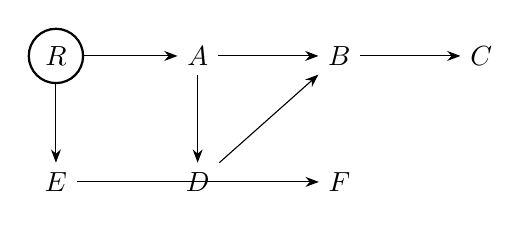
\begin{tikzpicture}[>=Stealth]
  \node[root] (R) at (0,0) {$R$};
  \node (A) at (1.8,0) {$A$};
  \node (B) at (3.6,0) {$B$};
  \node (C) at (5.4,0) {$C$};
  \node (D) at (1.8,-1.6) {$D$};
  \node (E) at (0,-1.6) {$E$};
  \node (F) at (3.6,-1.6) {$F$};

  \draw[->] (R) -- (A);
  \draw[->] (A) -- (B);
  \draw[->] (B) -- (C);
  \draw[->] (A) -- (D);
  \draw[->] (D) -- (B);
  \draw[->] (R) -- (E);
  \draw[->] (E) -- (F);
\end{tikzpicture}
\end{center}

\paragraph{Expansion algorithm:}
\begin{enumerate}
\item $\mathsf{frontier} = \{E\}$ (new successors of $R$), $r = 1$
\item Add $E$ with $\mathsf{rank}[E] = 1$
\item $\mathsf{frontier} = \{F\}$, $r = 2$
\item Add $F$ with $\mathsf{rank}[F] = 2$
\item $\mathsf{frontier} = \{\}$, done
\end{enumerate}

\paragraph{Result:} $\mathsf{current} = \{R, A, B, C, D, E, F\}$

\subsection{Example: Contraction (Removing an Edge)}

Now suppose we remove the edge $A \to D$.

\begin{center}
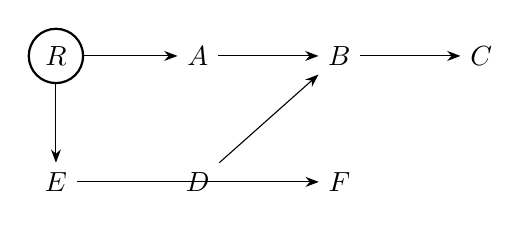
\begin{tikzpicture}[>=Stealth]
  \node[root] (R) at (0,0) {$R$};
  \node (A) at (1.8,0) {$A$};
  \node (B) at (3.6,0) {$B$};
  \node (C) at (5.4,0) {$C$};
  \node (D) at (1.8,-1.6) {$D$};
  \node (E) at (0,-1.6) {$E$};
  \node (F) at (3.6,-1.6) {$F$};

  \draw[->] (R) -- (A);
  \draw[->] (A) -- (B);
  \draw[->] (B) -- (C);
  \draw[->] (D) -- (B);
  \draw[->] (R) -- (E);
  \draw[->] (E) -- (F);
\end{tikzpicture}
\end{center}

\paragraph{Contraction algorithm:}
\begin{enumerate}
\item $\mathsf{worklist} = \{D\}$ (lost its incoming edge from $A$)
\item Process $D$:
  \begin{itemize}
  \item $D \notin \mathsf{base}$
  \item Check for wf-deriver: $\mathsf{stepInv}(D) = \{A\}$, but edge $A \to D$ removed
  \item No wf-deriver found, so $\mathsf{dying} = \{D\}$
  \item All dependents of $D$ already have another wf-deriver, so no additional nodes are added to the worklist
  \end{itemize}
\item $\mathsf{worklist} = \{\}$, done
\end{enumerate}

\paragraph{Result:} $\mathsf{current} = \{R, A, B, C, E, F\}$ (D removed)

\subsection{Example: Contraction with Cycles}

This example shows why \emph{ranks} are essential. Consider:

\begin{center}
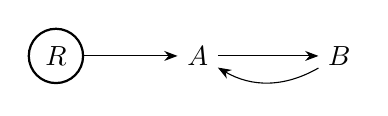
\begin{tikzpicture}[>=Stealth]
  \node[root] (R) at (0,0) {$R$};
  \node (A) at (1.8,0) {$A$};
  \node (B) at (3.6,0) {$B$};

  \draw[->] (R) -- (A);
  \draw[->] (A) -- (B);
  \draw[->] (B) to[bend left=30] (A);
\end{tikzpicture}
\end{center}

\begin{itemize}
\item $\mathsf{rank} = \{R \mapsto 0,\, A \mapsto 1,\, B \mapsto 2\}$
\item $A$ has a wf-deriver: $R$ with $\mathsf{rank}[R] = 0 < 1$
\item $B$ has a wf-deriver: $A$ with $\mathsf{rank}[A] = 1 < 2$
\end{itemize}

\paragraph{Now remove edge $R \to A$:}

\begin{center}
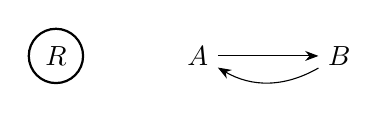
\begin{tikzpicture}[>=Stealth]
  \node[root] (R) at (0,0) {$R$};
  \node (A) at (1.8,0) {$A$};
  \node (B) at (3.6,0) {$B$};

  \draw[->] (A) -- (B);
  \draw[->] (B) to[bend left=30] (A);
\end{tikzpicture}
\end{center}

\paragraph{Contraction:}
\begin{enumerate}
\item $\mathsf{worklist} = \{A\}$ (lost edge from $R$)
\item Process $A$:
  \begin{itemize}
  \item $\mathsf{stepInv}(A) = \{R, B\}$
  \item $R \to A$ removed, so $R$ doesn't count
  \item $B$ is in current, but $\mathsf{rank}[B] = 2 > 1 = \mathsf{rank}[A]$ --- \textbf{not a wf-deriver!}
  \item No wf-deriver, so $A$ dies. Add $B$ to worklist.
  \end{itemize}
\item Process $B$:
  \begin{itemize}
  \item $\mathsf{stepInv}(B) = \{A\}$
  \item $A$ is dying, so doesn't count
  \item No wf-deriver, so $B$ dies.
  \end{itemize}
\item $\mathsf{worklist} = \{\}$, done
\end{enumerate}

\paragraph{Result:} $\mathsf{current} = \{R\}$ (entire cycle removed)

\paragraph{Key insight:} Without rank checking, $A$ and $B$ would keep each other alive (each derives the other). The rank check $\mathsf{rank}[y] < \mathsf{rank}[x]$ breaks this mutual support because cycle members have equal or increasing ranks along cycle edges.

\subsection{Summary}

\begin{center}
\begin{tabular}{|l|l|l|}
\hline
\textbf{Operation} & \textbf{Algorithm} & \textbf{Key Property} \\
\hline
Add edge/root & BFS expansion & Assigns increasing ranks \\
Remove edge/root & Worklist cascade & Rank check breaks cycles \\
\hline
\end{tabular}
\end{center}

\section{Level 2: DSL with Automatic Derivation (Future)}

The low-level API requires the user to provide $\mathsf{stepFromDelta}$ and prove that step is element-wise and additive.
A higher-level approach would let users define $F$ in a structured DSL, from which these properties are derived automatically.

\subsection{Analogy: Automatic Differentiation}

\begin{center}
\begin{tabular}{|l|l|l|}
\hline
& \textbf{Differentiation} & \textbf{Incremental Fixpoint} \\
\hline
Low-level & User provides $f(x)$ and $\frac{df}{dx}$ & User provides $F$, $\mathsf{stepFromDelta}$, proofs \\
\hline
High-level & User writes expression; & User writes $F$ in DSL; \\
(DSL) & system derives gradient & system derives incremental ops \\
\hline
Requirement & $f$ given as expression tree & $F$ given as composition of primitives \\
\hline
Black-box & Finite differences (slow) & Full recomputation (slow) \\
\hline
\end{tabular}
\end{center}

Just as automatic differentiation requires $f$ to be expressed as a composition of differentiable primitives, automatic incrementalization requires $F$ to be expressed as a composition of ``incrementalizable'' primitives.

\subsection{Potential DSL Primitives}

A DSL for fixpoint operators might include:
\begin{itemize}
  \item $\mathsf{const}(B)$: constant base set
  \item $\mathsf{union}(F_1, F_2)$: union of two operators
  \item $\mathsf{join}(R, S, \pi)$: join $S$ with relation $R$, project via $\pi$
  \item $\mathsf{filter}(P, S)$: filter $S$ by predicate $P$
  \item $\mathsf{lfp}(\lambda S. F(S))$: least fixpoint
\end{itemize}

Each primitive would come with:
\begin{itemize}
  \item Its incremental step function (for semi-naive)
  \item Its derivation counting semantics (for deletion)
\end{itemize}

\begin{example}[DCE in DSL]
\begin{verbatim}
live = lfp(S => 
  union(
    const(roots),
    join(edges, S, (u, v) => v)
  )
)
\end{verbatim}
The system derives:
\begin{itemize}
  \item $\mathsf{stepFromDelta}(\Delta) = \mathsf{join}(\mathsf{edges}, \Delta, (u,v) \mapsto v)$
  \item Proof that step is element-wise (each edge provides a single derivation)
  \item Proof that step is additive (union distributes over step)
\end{itemize}
\end{example}

\subsection{Connection to Datalog}

Datalog engines already perform similar derivations:
\begin{itemize}
  \item Rules are the structured representation of $F$
  \item Semi-naive evaluation is derived from rule structure
  \item Well-founded cascade generalizes deletion handling
\end{itemize}

A general incremental fixpoint DSL would extend this beyond Horn clauses to richer operators (aggregation, negation, etc.).

\section{Examples Beyond DCE}

The incremental fixpoint pattern applies to many problems:

\begin{center}
\begin{tabular}{|l|l|l|l|}
\hline
\textbf{Problem} & \textbf{Base} & \textbf{Step} & \textbf{Derivation Count} \\
\hline
DCE/Reachability & roots & successors & in-degree from live \\
\hline
Type Inference & base types & constraint propagation & \# constraints implying type \\
\hline
Points-to Analysis & direct assignments & transitive flow & \# flow paths \\
\hline
Call Graph & entry points & callees of reachable & \# callers \\
\hline
Datalog & base facts & rule application & \# rule firings \\
\hline
\end{tabular}
\end{center}

\section{Relationship to Reactive Systems}

In a reactive system like Skip:
\begin{itemize}
  \item \textbf{Layer 1} (reactive aggregation) handles changes to the \emph{parameters} of $F$ (e.g., the graph structure).
  \item \textbf{Layer 2} (incremental fixpoint) maintains the fixpoint as those parameters change.
\end{itemize}

The two layers compose: reactive propagation delivers deltas to the fixpoint maintainer, which incrementally updates its state and emits its own deltas (added/removed elements) for downstream consumers.

\section{Future Work}

\begin{enumerate}
  \item \textbf{Design Level 2 DSL}: Define a language of composable fixpoint operators with automatic incrementalization.
  
  \item \textbf{Integrate with Skip}: Implement the incremental fixpoint abstraction as a reusable component in the Skip reactive framework.
  
  \item \textbf{Explore stratification}: Extend to stratified fixpoints (with negation) where layers must be processed in order.
  
  \item \textbf{Benchmark}: Compare incremental vs.\ recompute performance on realistic workloads.
\end{enumerate}

\section{Conclusion}

The incremental DCE algorithm is an instance of a general pattern: maintaining least fixpoints incrementally under changes to the underlying operator.
We propose a two-level architecture:
\begin{enumerate}
  \item A \textbf{low-level API} where users provide \textsf{stepFromDelta} and prove step is element-wise and additive.
  \item A \textbf{high-level DSL} (future work) where these proofs are derived automatically from a structured definition of $F$, analogous to how automatic differentiation derives gradients from expression structure.
\end{enumerate}

The key contribution is \emph{well-founded cascade}: using the iterative construction rank to handle cycles correctly. Elements not in the new fixpoint have no finite rank, so they have no well-founded derivers and are removed.

This abstraction unifies incremental algorithms across domains (program analysis, databases, reactive systems) and provides a foundation for building efficient, correct incremental computations.

\end{document}
